\section{Discussion}

\begin{figure}
\centering 
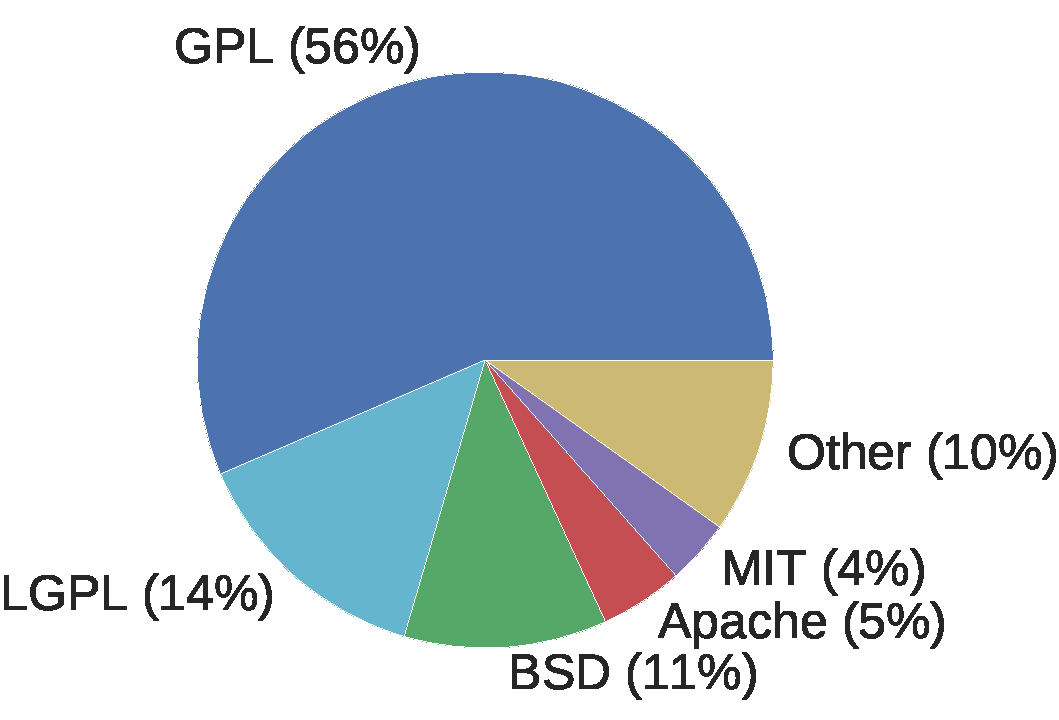
\includegraphics[width=.5\linewidth]{../licenses}
\caption{\label{licenses} Distribution of open-source licenses used in cataloged software packages.}
\end{figure}

\begin{figure*}
\centering
\begin{subfigure}[t]{.4\linewidth}
\centering \label{develop}
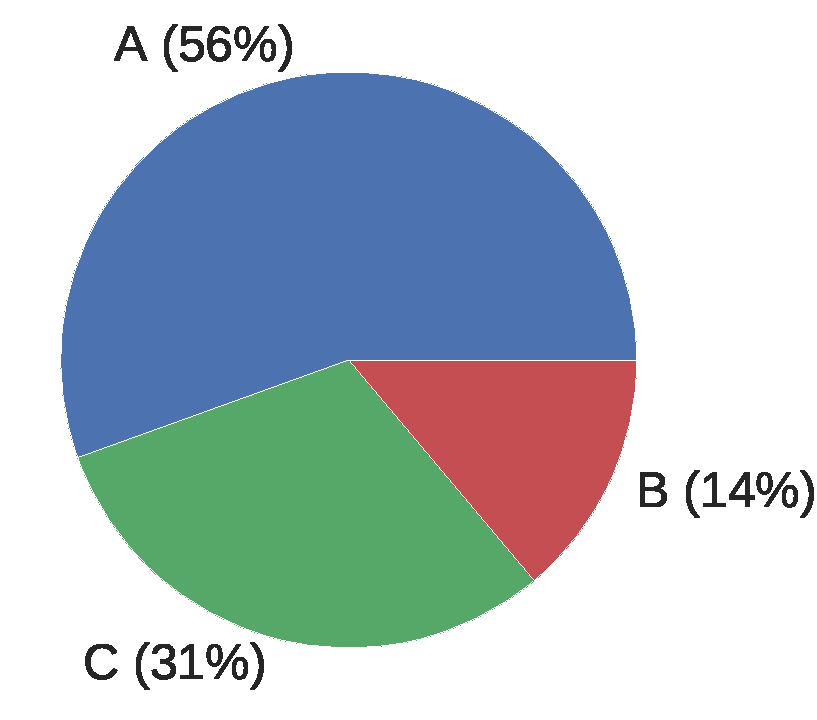
\includegraphics[width=\linewidth]{../develop}
\end{subfigure}
\hfill
\begin{subfigure}[t]{.4\linewidth}
\centering \label{usage}
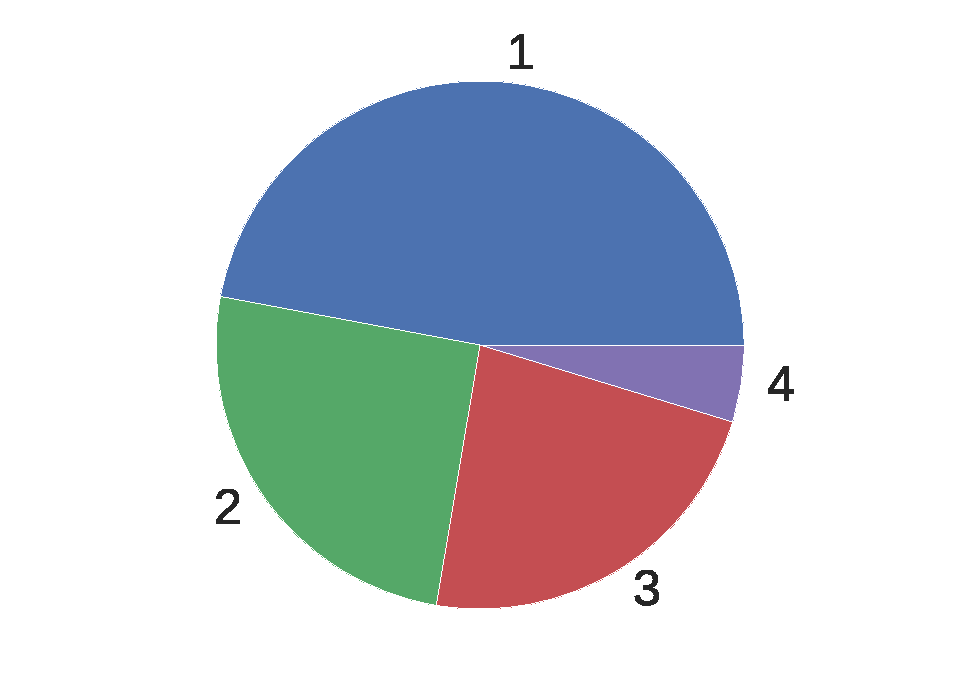
\includegraphics[width=\linewidth]{../usage}
\end{subfigure}
\caption{\label{pies} Activity distributions of cataloged software packages.
\subref{develop} Distribution of development activity. \subref{usage} Distribution of user activity.
}
\end{figure*}

\begin{figure}
\centering 
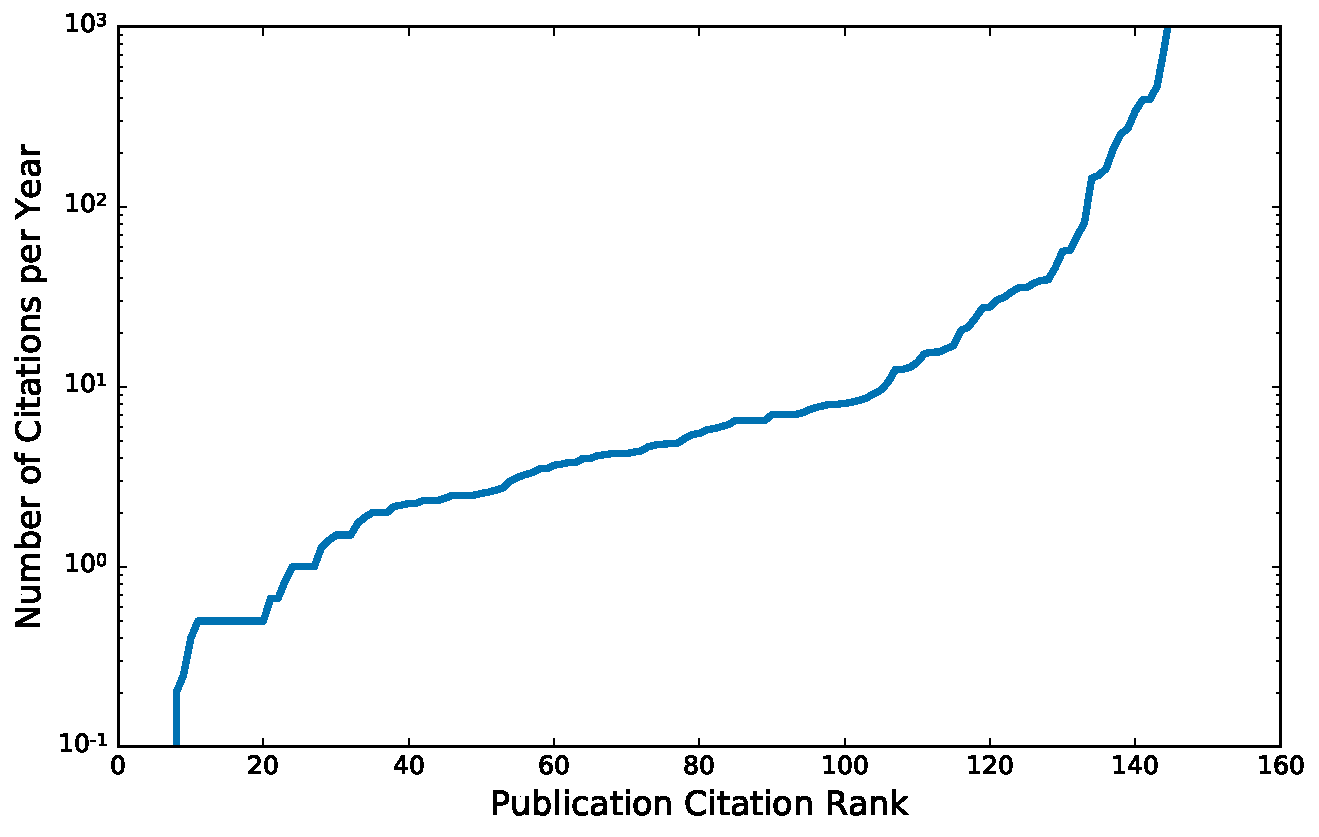
\includegraphics[width=.5\linewidth]{../citedist}
\caption{\label{cites} Distribution of citations as reported by Google Scholar generated on average every year by those software packages with citeable publications.}
\end{figure}


We have cataloged \textbf{X} open-source packages for molecular modeling that provide a wide range of capabilities.  As shown in Figure~\ref{licenses}, the most popular license (\textbf{X\%}) is some variant of the copyleft GNU Public License, which ensures that derivative works remain open source.  Interestingly \textbf{X\%} of the packages catalog have a corresponding, citeable publication which suggests that much of the software originates from academia.   The distribution of average citations generated a year (as reported by Google Scholar) for the citeable publications is shown in Figure~\ref{cites}.  The majority of publications generate at least one citation a year, and about 10\% generate more than 50 a year.

A substantial portion of the packages cataloged are under active development and see significant usage, as shown in Figure~\ref{pies}.  We rated \textbf{X\%} of the packages as `A' level development, meaning major features or releases were made within the last 18 months, and \textbf{X\%} see substantial usage (rank 1).  
There a number of projects (\textbf{X\%}) where development has apparently ceased (no changes within the last 18 months). Note our methodology for identifying packages eliminates complete abondonware, so this is an underestimate.  However, anecdotally although we did find instances where an open source package was referenced in a paper but was no longer available, we did not find this to be a common occurance.  Most packages, even those that have remained unchanced for a decade, see some usage.  In fact, a number of packages (\textbf{X}), still see significant usage despite having received no development for the past 18 months.  This underlies the importance of releasing source code through a third-party site such as SourceForge or GitHub as it ensures the continued existence of a project.  A major advantage of open source is that in cases where a popular project is not being actively developed (e.g. AutoDock Vina) new projects can fork the source code and continue development (e.g. smina).

It is clear that open source software plays an important role in the scientific community and is a vibrant sub-community of as own with a wide assortment of projects under development and in widespread use.  The open source software packages cataloged here provide launching points for the development of new tools for enabling further scientific discovery.
